
\subsection{Evaluation of the classification of tweets}
Evaluation is one of the most important part of a categorization process because it tells if the classification behaves as desired. Classification is, as already mentioned, difficult to evaluate and it was therefore quite useful to look at the evaluation part of the classification of tweets.

The authors argued that the computer classification should be compared by classification done by humans, so that the \textit{predicted} result could be compared with the \textit{correct} result. The problem is that it is very time consuming for humans to classify, so the evaluation was done by sampling 500 tweets. Of these tweets were 477 manually identified by people to give them tags which were compared by the classifier's tags. 

Figure \ref{fig:classification_entities} shows the results of the evaluation phase of the classification. The measures for each tag are P (precision: fraction of retrieved tweets that are relevant), R (recall: fraction of relevant tweets that were tagged) and F1 (F1-score: measure of accuracy, given as $ F_1 = 2 \cdot \frac{\mathrm{precision} \cdot \mathrm{recall}}{\mathrm{precision} + \mathrm{recall}}$). It is interesting to look at the results from the evaluation because they give a good indication on which subjects are difficult to classify. The results show that people and locations are easy to classify, while music is more difficult. This could be because music might contain common words that are dropped from the knowledge base or does not provide useful information while name of locations are easy to recognize for the classifier. 
%One of the most important steps of classifying is the evaluation phase. Evaluation of classifying should be done by humans. Someone will have to look through the results and see how well the classification has been done by comparing the \textit{correct} result with the \textit{predicted} result.

%The article concludes that the tweets that were easiest to classify were about people (see Figure \ref{fig:classification_entities}). This is probably because famous people have their own Wikipedia page, which is easy to match the tweet. The most difficult, on the other hand, was products which seldom have their own page  if the tweet is very specific. 


\begin{figure}[H]
\centering
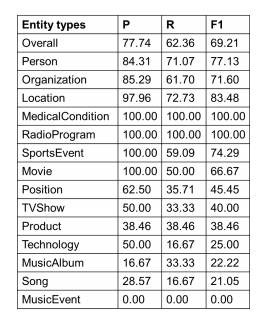
\includegraphics[height=8cm]{Classification_entities}
\caption{The accuracy of the system for extraction and linking.}
%P is the precision, R is the recall and $F_{1}$ is the $F_{1}$-score.} %linking\footnote{\url{http://pages.cs.wisc.edu/~anhai/papers/doctagger-vldb13.pdf, page 8}}}
\label{fig:classification_entities}
\end{figure}